%--------------------------------------------------
\subsection{Prototipo 4: Prototipo final }

El prototipo final de la aplicación incluye la actualización de las vistas finales de la aplicación, así como las últimas modificaciones que se realizaron para la integración de la aplicación con Firebase Cloud Messaging para el envío y recepción de notificaciones. \\ \par

%--------------------------------------------------

\subsubsection{Análisis}

Dentro del análisis de este prototipo se realiza la inclusión del siguiente requerimiento funcional a los ya definidos previamente en el capítulo del ``Bosquejo general de la aplicación''  con el título de \hyperlink{RFAPV}{``Requerimientos Funcionales de la Aplicación Interactiva para el Personal de Ventas''}:\\

\begin{itemize}
\item Actualizar token de Firebase Cloud Messaging (FCM)
\end{itemize}

\hypertarget{NRFAPV}{}
\begin{FRequirements}
\FRitem{RFAIPV7}{Actualizar token de Firebase Cloud Messaging (FCM)}{
La aplicación permitirá actualizar el token de FCM para subscribirse a las notificaciones de cada uno de los departamentos a los que el vendedor se dirija, es decir, cada que el vendedor cambie de departamento de igual forma lo hará el token.
}
\caption{Requerimiento añadido a los Requerimientos Funcionales de la Aplicación Interactiva para el Personal de Ventas.}
\end{FRequirements}

\paragraph{Casos de uso de la AIPV.} ~\\

La figura \ref{casos-uso-AIPVFinal} muestra las modificaciones finales de los casos de uso de la AIPV, en la siguiente lista se detalla cuales fueron.

\begin{itemize}
\item CUAPV4 Obtener localización aproximada del cliente fue modificado y ahora es CUAPV4 Obtener detalles y estadísticas del cliente, entre los detalles del cliente se indica en que departamento y a que hora se encontraba en el cliente.
\item CUAPV5 Obtener estadísticas del cliente fue eliminado ya que dichas estadísticas se obtienen en conjunto con los detalles y en su lugar se encuentra ahora el CUAPV5 Actualizar token de Firebase Cloud Messaging (FCM) para controlar la suscripción de notificaciones del vendedor dependiendo del departamento en el que se encuentre.
\end{itemize}

\FloatBarrier
\begin{figure}[htbp!]
		\centering
			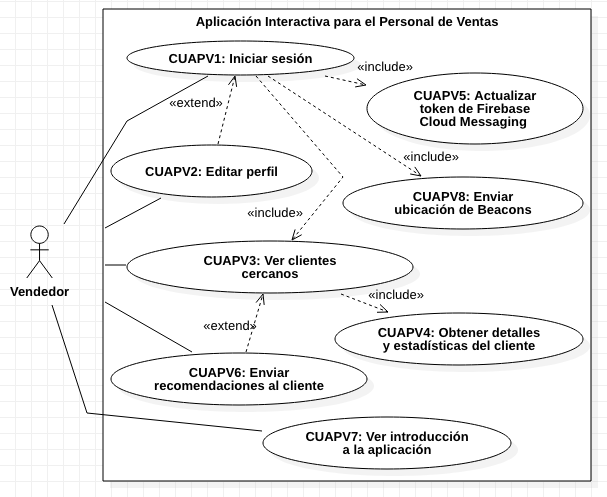
\includegraphics[width=.8 \textwidth]{imagenes/adrian/vendedor/prototipoFinal/casosDeUso}
		\caption{Casos de uso de la AIPV.}
		\label{casos-uso-AIPVFinal}
\end{figure}
\FloatBarrier

%--------------------------------------------------
\subsubsection{Diseño}

%introducción%
A continuación se muestra el diagrama de secuencia para actualizar el token de FCM, el flujo de navegación y el diseño final de las interfaces de la aplicación.\\ \par

\paragraph{Diagramas de secuencia.} ~\\

\title{\textbf{Actualizar el token de FCM.}\\}

En la figura \ref{secuencia-AIPV4-token} se muestra el diagrama de secuencia para actualizar el token de FCM, el cual describe los pasos que se llevan a cabo cada que el vendedor se encuentra dentro de la zona de proximidad de un Beacon de diferente departamento al anterior, esto para mantenerlo suscrito a las notificaciones del departamento actual. Para una mejor visualización el diagrama se ha dividido en 3 partes las cuales se muestran en las figuras \ref{secuencia-AIPV4-tokenUno}, \ref{secuencia-AIPV4-tokenDos}  y \ref{secuencia-AIPV4-tokenTres} .

\FloatBarrier
\begin{figure}[htbp!]
		\centering
			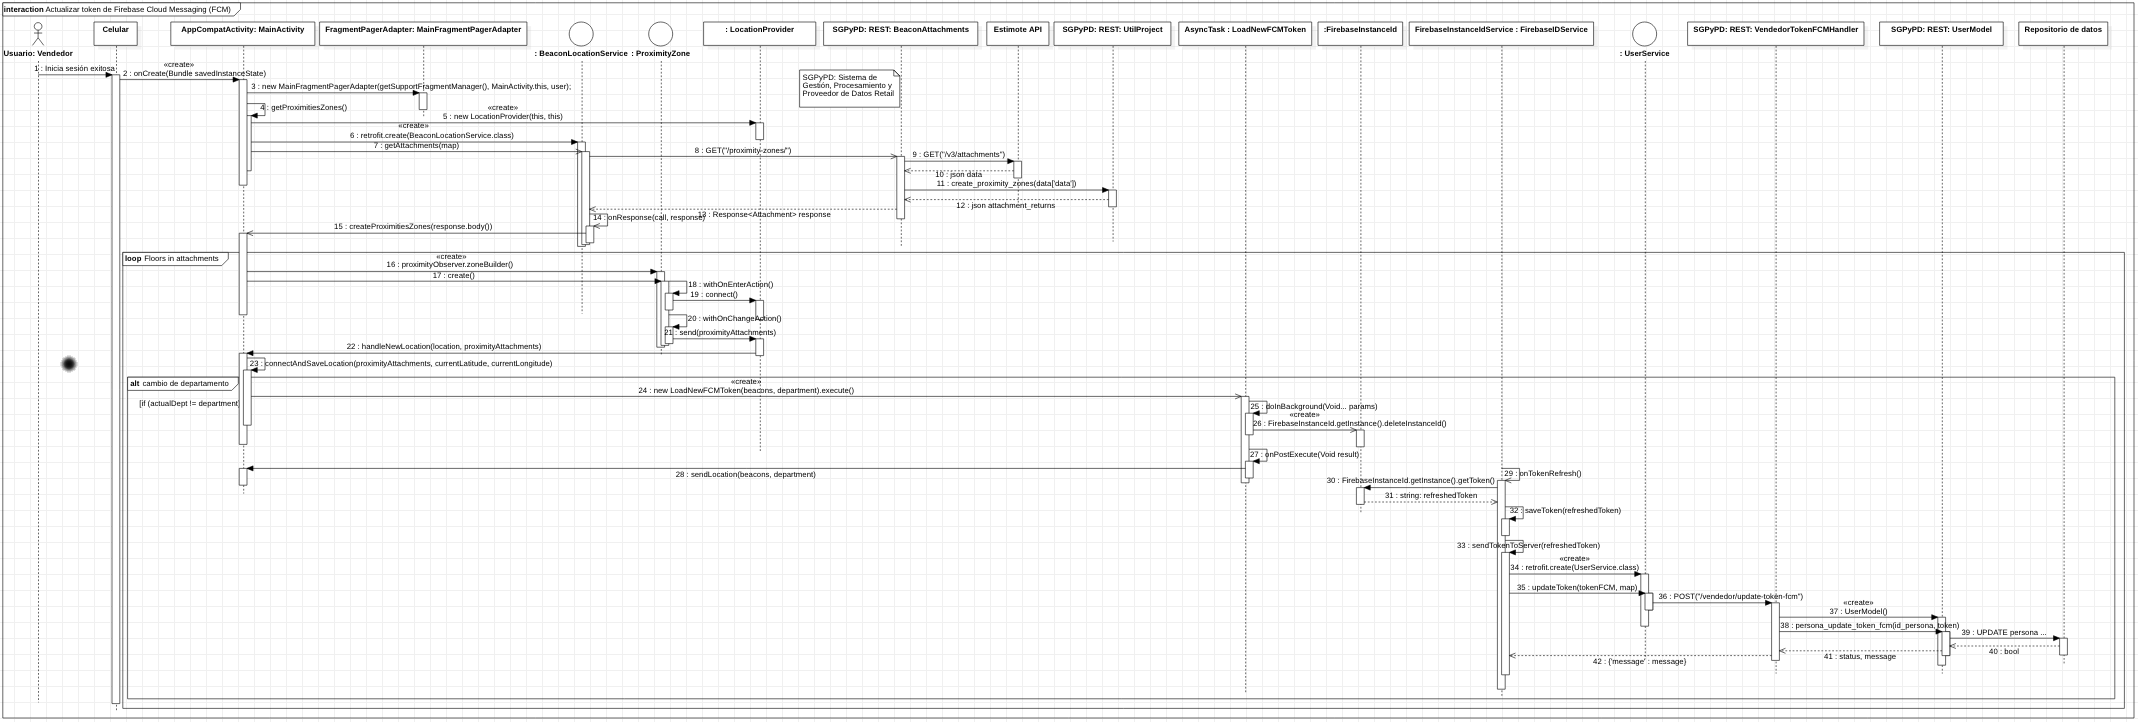
\includegraphics[width=1 \textwidth]{imagenes/adrian/vendedor/prototipoFinal/actualizarFCM}
		\caption{Diagrama de secuencia para actualizar el token de FCM.}
		\label{secuencia-AIPV4-token}
\end{figure}
\FloatBarrier

\FloatBarrier
\begin{figure}[htbp!]
		\centering
			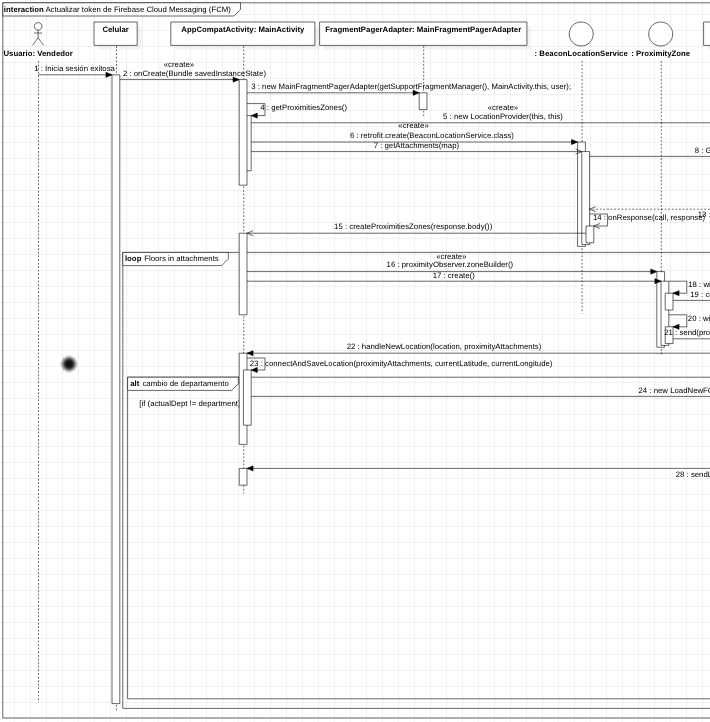
\includegraphics[width=1 \textwidth]{imagenes/adrian/vendedor/prototipoFinal/actualizarFCM1}
		\caption{Diagrama de secuencia para actualizar el token de FCM (Parte 1).}
		\label{secuencia-AIPV4-tokenUno}
\end{figure}
\FloatBarrier

\FloatBarrier
\begin{figure}[htbp!]
		\centering
			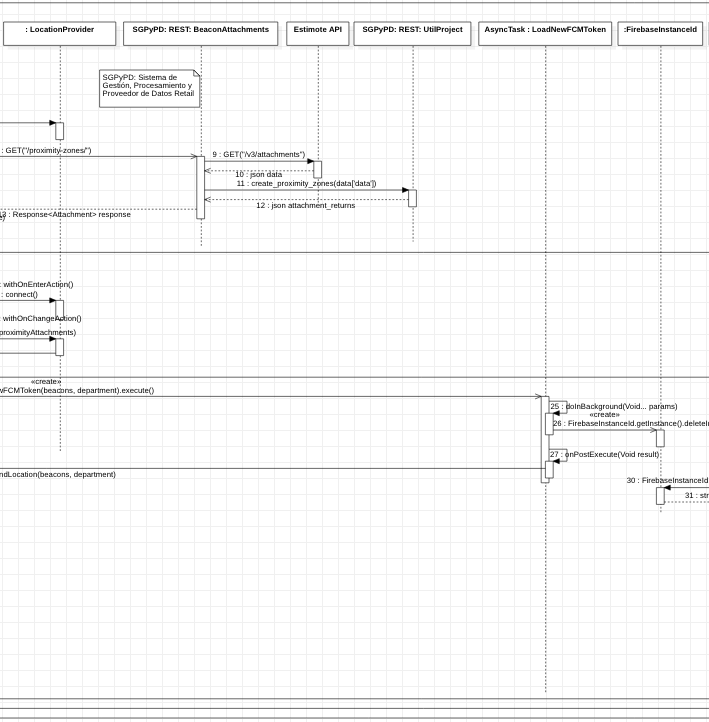
\includegraphics[width=1 \textwidth]{imagenes/adrian/vendedor/prototipoFinal/actualizarFCM2}
		\caption{Diagrama de secuencia para actualizar el token de FCM (Parte 2).}
		\label{secuencia-AIPV4-tokenDos}
\end{figure}
\FloatBarrier

\FloatBarrier
\begin{figure}[htbp!]
		\centering
			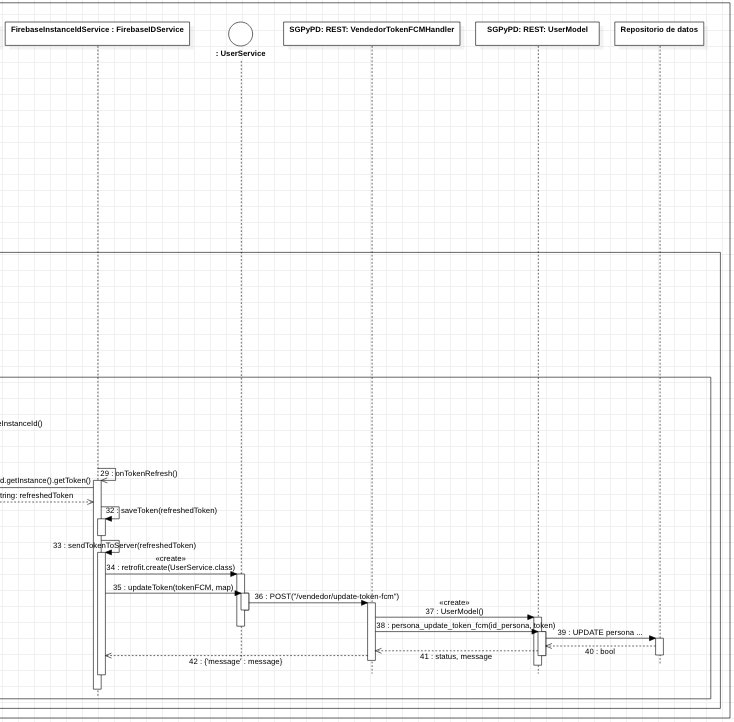
\includegraphics[width=1 \textwidth]{imagenes/adrian/vendedor/prototipoFinal/actualizarFCM3}
		\caption{Diagrama de secuencia para actualizar el token de FCM (Parte 3).}
		\label{secuencia-AIPV4-tokenTres}
\end{figure}
\FloatBarrier
%Redactar modificaciones que se hicieron 

\paragraph{Flujo de navegación final de la AIPV.} ~\\

La siguiente figura \ref{navegacion-AIPVFinal} muestra como es el flujo final de navegación de la aplicación.

\FloatBarrier
\begin{figure}[htbp!]
		\centering
			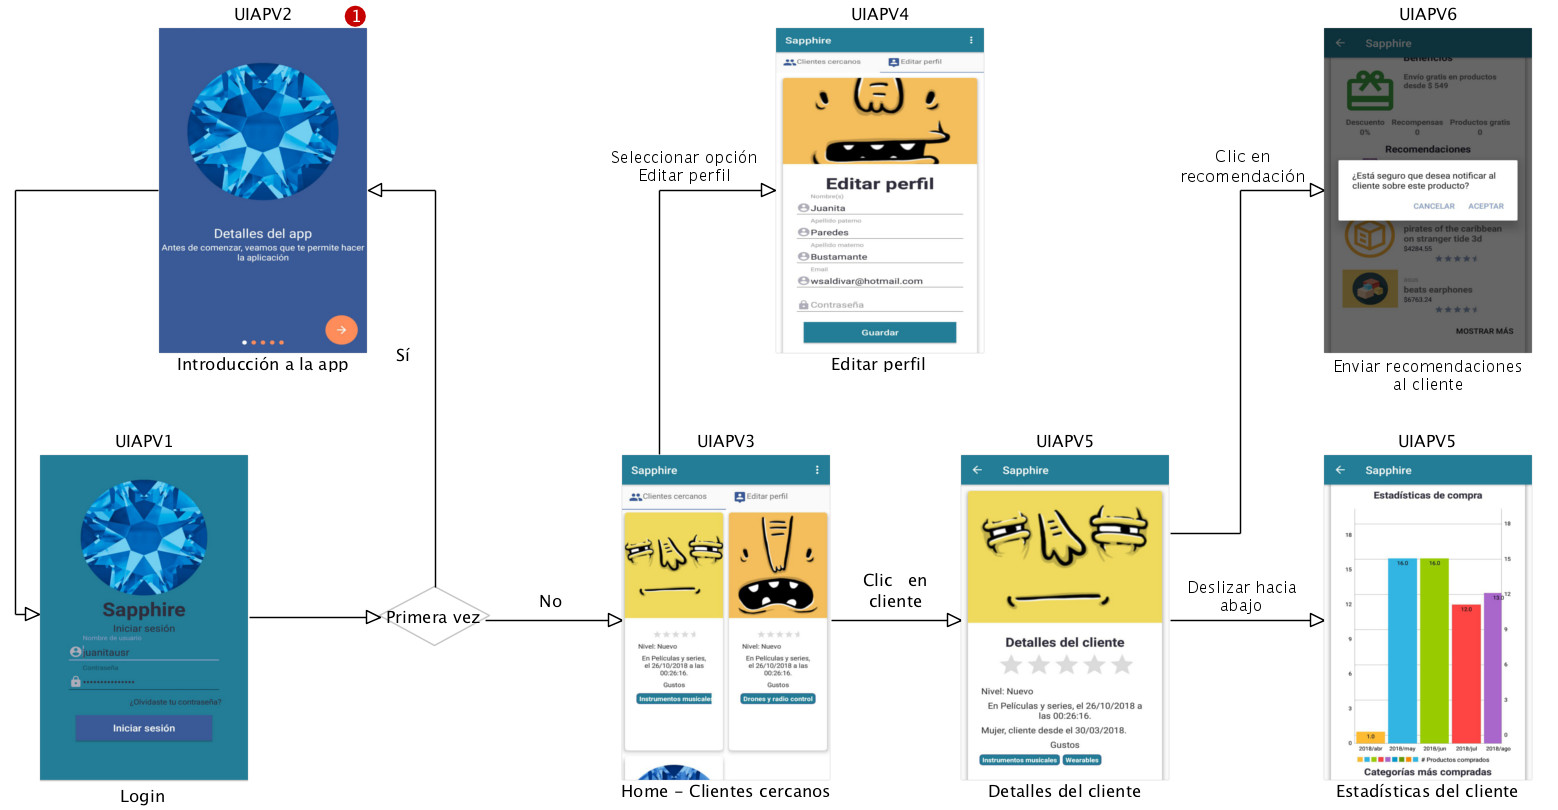
\includegraphics[width=1 \textwidth]{imagenes/adrian/vendedor/prototipoFinal/UIApp/ui}
		\caption{Flujo final de navegación de la AIPV.}
		\label{navegacion-AIPVFinal}
\end{figure}

\paragraph{Interfaces de usuario}

\cfinput{appMovil/Vendedor/UIFinal/UIAPV1}
\cfinput{appMovil/Vendedor/UIFinal/UIAPV2}
\cfinput{appMovil/Vendedor/UIFinal/UIAPV3}
\cfinput{appMovil/Vendedor/UIFinal/UIAPV4}
\cfinput{appMovil/Vendedor/UIFinal/UIAPV5}
\cfinput{appMovil/Vendedor/UIFinal/UIAPV6}
\cfinput{appMovil/Vendedor/UIFinal/UIAPV7}

%--------------------------------------------------
%\subsubsection{Pruebas}